\documentclass[oneside,11pt]{amsart}
\usepackage[utf8]{inputenc}%
\usepackage[english]{babel}%
\usepackage{amsmath,amssymb,amsthm,amsfonts}%
\usepackage[unicode]{hyperref}%
\usepackage{mathrsfs,bbm}%
\usepackage{paralist}
\usepackage{color}
\usepackage{longtable}
\usepackage{array}
\usepackage{stmaryrd}%
%\usepackage{refcheck}
\usepackage{graphicx}
\usepackage[DIV15]{typearea}
\usepackage{multicol,tikz}
\usepackage{datetime}
\usepackage{cleveref}

\usepackage[shadow]{todonotes}

\usepackage{etoolbox}
\patchcmd{\section}{\scshape}{\large\itshape\bfseries}{}{}

\usepackage{caption}
\captionsetup{labelformat=empty,labelsep=none}

\hypersetup{
  colorlinks=true,
  linkcolor=blue!50!red,
  urlcolor=green!60!black
}

%%%%%%%%%%%%%%%%%%%%%%%%%%%%%%%%%%%%%%%%%%%%%%%%%%%%%%%%%%%%%%%%%%%%%%%%%%%%%%%%%%%%%%%%
\synctex=1
%%%%%%%%%%%%%%%%%%%%%%%%%%%%%%%%%%%%%%%%%%%%%%%%%%%%%%%%%%%%%%%%%%%%%%%%%%%%%%%%%%%%%%%%
%%%%%%%%%%%%%%%%%%%%%%%%%%%%%%%%%%%%%%%%%%%%%%%%%%%%%%%%%%%%%%%%%%%%%%%%%%%%%%%%%%%%%%%%

\begin{document}

\title[Building Truth from Scratch]{EGMT 1520: Building Truth from Scratch\\(Empirical \& Scientific Engagement)}
\author{Leonid Petrov\\Fall 2025}
\date{Compiled on \today, \currenttime. An up to date syllabus is always at \href{https://github.com/lenis2000/Syllabi/blob/master/Syllabus_EGMT_f25.pdf}{\texttt{this link}}.}
\maketitle


\section{How do we know a claim is true?}

This course is a hands-on workshop in making and testing arguments in the context of mathematics.
We will generate conjectures from examples, search for counterexamples, and turn ideas into precise statements and proofs. Through problem-solving sessions and math debates, you'll practice evaluating arguments, giving and receiving constructive feedback, and communicating clearly in writing and speech. By experiencing mathematics as a creative process --- where patterns suggest conjectures and logical reasoning turns intuition into conviction --- you'll develop a practical sense for what counts as evidence in mathematics and how to build reliable conclusions.
By the end of the course, you will be able to
\begin{enumerate}[$\bullet$]
    \item \textbf{Define and delimit what constitutes valid mathematical evidence} by distinguishing between examples, counterexamples, conjectures, and formal proofs, while recognizing the limitations of empirical observations.
    % \emph{(Aligned with pillar objective: “define and delimit what constitutes empirical evidence”)}
    \item \textbf{Develop a framework for discerning different types of mathematical knowledge} by exploring how empirical evidence, abstract reasoning, and logical structure work together to shape mathematical understanding.
    % \emph{(Aligned with pillar objective: “develop a framework for discerning types of knowledge based on what is empirically
% observable in the natural, physical and social worlds”)}
    \item \textbf{Formulate and communicate mathematical reasoning} by translating intuitive insights into precise statements, evaluating the soundness of arguments, and engaging in constructive dialogue to identify and resolve reasoning gaps.
    % \emph{(Aligned with pillar objective: “evaluate supported claims about the natural and social worlds by framing empirical questions and methods and interpreting the claims in the context of new data”)}
    \item \textbf{Reflect on the nature of mathematical truth} by examining personal assumptions about certainty, analyzing when and why certain arguments are conclusive, and articulating how purely empirical approaches can both inform and limit our understanding of complex phenomena.
    % \emph{(Aligned with pillar objective: “articulate the limitations of using only empirical approaches to describe complex phenomena”)}
\end{enumerate}

\begin{center}
\vspace{1cm}
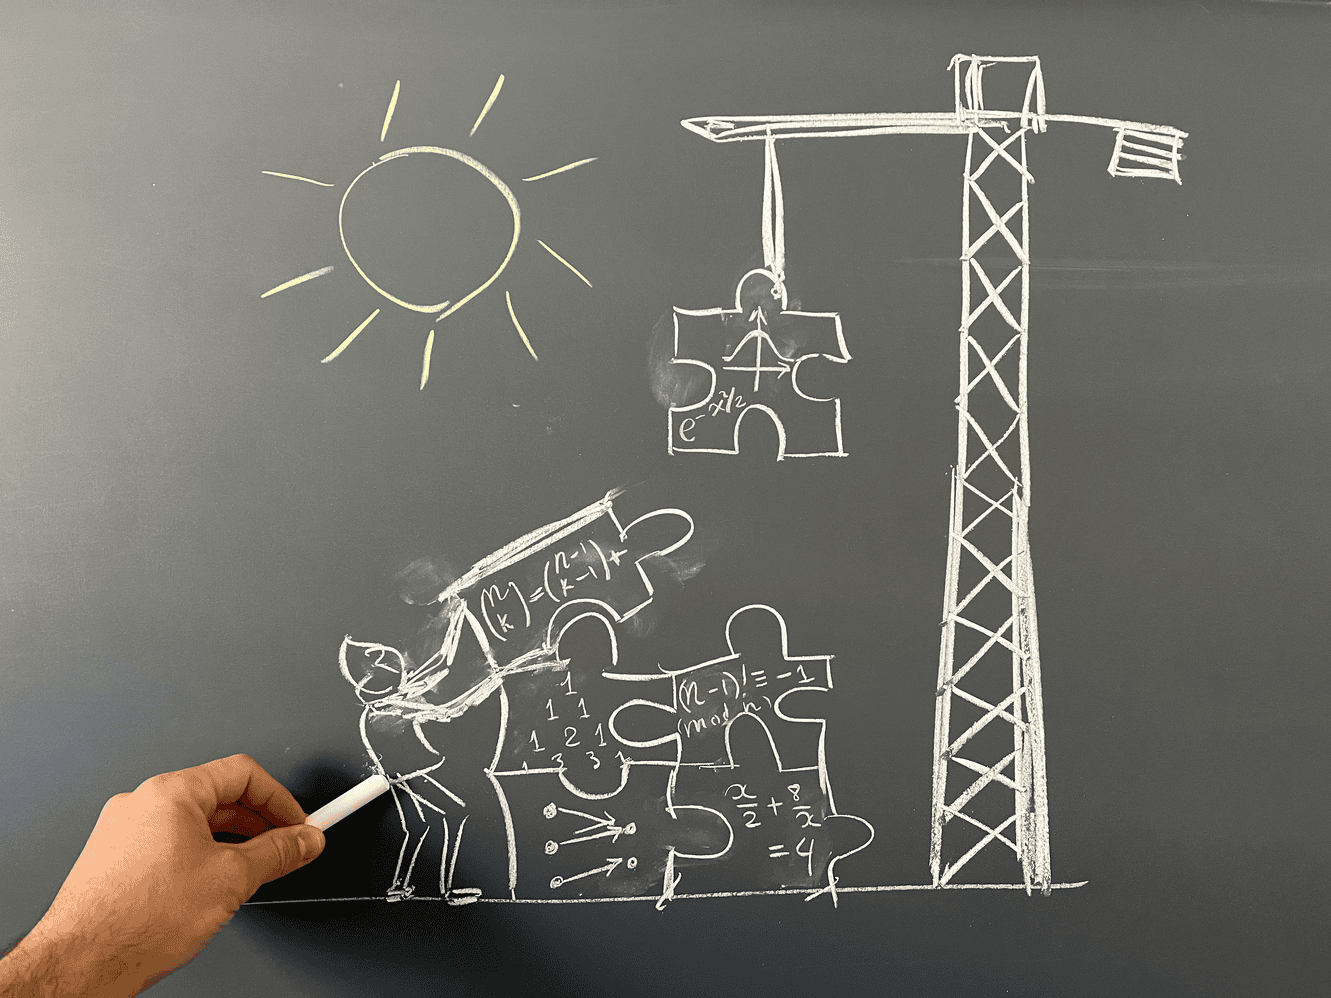
\includegraphics[width=.5\textwidth]{EGMT_image.png}
\vspace{1cm}
\end{center}

\newpage
\section{Contact \& Logistics}

\noindent
\begin{tabular}{ll}
\textbf{Instructor:} Leonid Petrov &\qquad \qquad \qquad\textbf{Office:} 209 Kerchof Hall \\
\textbf{Email:} \href{mailto:petrov@virginia.edu}{petrov@virginia.edu} & \qquad \qquad \qquad\textbf{Office hours (from Sep 1):} \\
\textbf{Website:} \url{https://lpetrov.cc}
& \qquad \qquad \qquad Mon 11:30am--12:30pm, Thu 10:30--11:30am \\
& \qquad \qquad \qquad or by appointment (email me; you can make \\
& \qquad \qquad \qquad as many appointments as you need)
\end{tabular}

\smallskip
\noindent\textbf{Weekly rhythm:} Class meets Mondays
3:30--6:00PM, Gilmer Hall 247
(September 1, 8, 15, 22, 29; October 6).
Your single weekly submission (two reflections + one designated problem write-up) is due on \textbf{Sunday 10:00\,pm} on Canvas.

\smallskip
\noindent
\textbf{Math debate split session:}
In addition, each student will attend one of two math debate sessions. I plan two
sessions, in the weeks of September 15 and 22. The timing will be
determined by polling the class on their availability.

\smallskip
\noindent
\textbf{Course materials:}
There are no required textbooks for this course.
All materials will be handed out in class and later posted on Canvas.
The Commonplace Book is an integral part of the course for homework assignments and reflections,
and it is required that you bring it to class each week, and to the math debate.

\section{How we work together in class}

This is a hands-on, pen-and-paper course.
The weekly meetings have roughly the same structure.

\subsection{Weekly meeting structure}

Each meeting begins with
a brief review, then you receive
a fresh problem set. You work at your table in fixed small subgroups, develop ideas, test them, and revise when needed. I circulate, ask questions, and may invite nearby peers to listen in and
challenge your reasoning.

\begin{enumerate}[$\bullet$]
  \item \textbf{Home subgroups (fixed):} On day one we form 6 ``home subgroups'' for in-class collaboration:
  $\delta, \ \theta, \ \zeta, \ \rho, \ \lambda, \ \phi$.\footnote{Math and science use Greek symbols very often. The names of the subgroups are
	\emph{delta}, \emph{theta}, \emph{zeta}, \emph{rho}, \emph{lambda}, and \emph{phi}.}
	Subgroups remain stable.

  \item \textbf{In-class problem work (at the table):} At
	the start of class you receive a new problem set.
	Your group works at the table; when ready, you explain
	your solution to me. I act as a skeptical audience.
	You may use scrap paper or your Commonplace Book to write up your solution.\footnote{The pages
	in the Commonplace Book are probably not enough for all work throughout the semester. I will bring
	a lot of scrap paper to class. I ask to complete homework assignments in the Commonplace Book, and
	submit photos to Canvas.}
	During your subgroup's explanation, I may ask a different member to continue the explanation,
	so everyone should understand the full argument.

  \item \textbf{Random mixers:}
		Near the end of class, we spend about 10-15 minutes
		in randomly mixed groups.
		Quick reshuffles outside your home group allow you
		to compare partial solutions and share techniques.

	 \item \textbf{Mini-debate session (dedicated slot with a new
	 problem):} In a scheduled debate block (separate from
	 regular weekly work), the class receives a {new}
	 problem designed for argument-testing. There is
	 structured {work time} to develop approaches,
	 followed by {presentation and questioning}.
	 A pair of presenters will be at the board explaining the
	 solution, while the rest of the class
	 focuses on questioning and debating the claim.

	\item \textbf{Math debate:} Scheduled separately; see below for details.

	\item \textbf{Commonplace book:} Bring it every time.
	Use it to capture mathematical beauty you will see in class, and for
	some of the required in-class work.
	Photos of selected pages
	are submitted to Canvas each week (see details below).

  \item \textbf{Team roles (rotate each meeting):} In subgroups of $5$--$6$,
		the following sample roles work well:
		\begin{compactitem}
			\item \textsc{Explainer}: articulates the current
			approach and restates the problem in your own words.
			\item \textsc{Skeptic}: presses on assumptions, looks
			for gaps, and frames precise questions.
			\item \textsc{Counterexample Hunter}: designs and
			tests examples/edge cases to probe the claim.
			\item \textsc{Recorder}: maintains a clean write-up of the
			steps in the problem.
			\item \textsc{Verifier}: checks computations and logic, and
			ensures steps follow from the stated problem.
			\item \textsc{Connector}: ensures that all subgroup
			members understand and can explain the solution.
		\end{compactitem}
		You may keep the roles informal or explicitly assign them in your
		subgroup, but \emph{make sure you rotate them at least each week,
		if not more often}.

	\item \textbf{Topic:}
		The weekly math topic is not announced in advance --- we
		need everyone to bring their curiosity and creativity to
		the class for a shared joy of discovering new ideas.

  \item \textbf{Devices:} Please keep devices in your bag
		unless you have an accommodation that requires otherwise.
		This is a pen-and-paper course.
\end{enumerate}



\subsection{Advising}
Each meeting will also include a 20-minute advising activity, which is an integral part of the Engagements program in the first quarter.
Examples of the activities:
\begin{enumerate}[$\bullet$]
\item Reading the syllabus, and immediate advising questions (first meeting);
\item How to address professors in person and in email;
\item Study skills;
\item The role of letters of recommendation, undergraduate research, and how to connect to your professors;
\item Guest presentations.
\end{enumerate}


\section{Commonplace Book weekly assignments}

Each week after the class,
you will need to complete a three-part assignment in your Commonplace Book,
and submit photos of the pages to Canvas.

\begin{enumerate}[(1)]
  \item
	\textbf{Weekly reflection (300 words / 1 page limit)} --- question changes
	every week. Examples:
	\begin{enumerate}
	\item
		\textbf{What is the hardest mathematical fact I have ever seen and understood
		in my life?}
		(\emph{this is the pre-class assignment, due on August 31}).
		Describe your mathematical journey in your own words (not just list
		math classes you took). What was the hardest mathematical thing you
		have ever seen and understood?
		\emph{This assignment will help me form balanced home subgroups.}
	\item
		\textbf{What counted as evidence for me?}
		Name one math experience from this week
		and list \emph{exactly what} made it convincing \emph{to
		you} (e.g., a minimal example, a failed counterexample, a
		definition that removed ambiguity, an auxiliary statement
		that closed a gap).
		End with one thing that would change your mind about
		this experience being convincing.
	\item \textbf{Reflect on the nature of mathematical truth.}
		What does it mean for a mathematical claim to be true?
		How is it different from a scientific claim, like
		``water boils at 100 degrees Celsius''?
		What is the role of examples, counterexamples, and proofs
		in establishing mathematical truth?
		How the math debate participants used mathematical truth to communicate
		what really is going on in a given setup?
	\end{enumerate}

  \item \textbf{Assumption audit (300 words / 1 page limit)}
	Pick one problem from the problem set, and list all
	assumptions you used in your solution
	(not just those stated in the problem). For each, mark:
	\emph{needed} / \emph{not needed} / \emph{uncertain}. Then
	try to \emph{drop one}: either give a tiny counterexample
	that shows it \emph{was} needed, or a brief note
	explaining why the argument still goes through.

  \item \textbf{Complete solution write-up (one problem)}
  Choose one problem \emph{designated for write-up} in the handout, and write a clear, self-contained solution. Define terms you use, justify each step, and cite any previously settled claims.
\end{enumerate}
\emph{Submission format:} Clear photos or a single PDF to Canvas by \textbf{Sunday 10:00\,pm}, submitted to the required assignment.

\medskip\noindent
Note: It is helpful to also bring your Commonplace Book to class,
to keep your homework in one place, as well as to put important
advising information there.


\section{Math debate}

The math debate is a structured two-team activity.
The teams consist of 8-9 students and are separate from the
in-class subgroups. The class is split into four teams of 8-9 people,
two for each debate session.
The other teams are very welcome to attend the debate, too.
Splitting into teams will happen on September 15, the third class meeting.

The debate has the following structure:
\begin{enumerate}[$\bullet$]
\item \textbf{0:00--0:10} --- Welcome briefing and choosing the
team that calls first by
a
1-minute mini-problem (any teammate may answer; the team, not a person, wins initiative). After Round~1, initiative alternates.

\item \textbf{0:10--1:10} | An hour of problem solving. Same packet
is issued to both teams, and they collaborate in their own rooms or spaces.
Teams decide internally who will present which problem.
Each team member can present at most once.
The teams also select a liaison for each round, who will announce the challenge.

\item \textbf{1:05--1:10} | Lock (finalize): answers. Submit brief answer slips (claims/ideas only).

\item \textbf{1:10--2:20} |
Three rounds of debate.
Suppose Team~A has the initiative.
Current round liaison from Team~A
announces the problem.
There are two outcomes:
\begin{enumerate}
\item If Team~B accepts the challenge, they present their solution
(6 minutes max) $\to$
Team~A asks up to 2 questions (2 minutes max)
$\to$
Team~B then presents their opposition (5 minutes max)
$\to$
Team~A replies to the opposition (3 minutes max).
\item If Team~B rejects the challenge, roles change, and Team~A presents their solution (6 minutes max) $\to$
Team~B asks up to 2 questions (2 minutes max)
$\to$
Team~A then presents their opposition (5 minutes max)
$\to$
Team~B replies to the opposition (3 minutes max).
\end{enumerate}
For each round, there is one person from each team at the board. Each person
may be at the board at most once per the whole debate.
In each round, every team has a 30-sec timeout to consult with their presenter. Outside of the timeout, the teams and the audience must be silent.

\item Scoring is 12 points per round,
split between the two teams and ``the audience'':\footnote{Team scores
in the math debate
don't affect the course grade.}
\begin{enumerate}
\item \textbf{Presenting team (0--12):} Correctness \& completeness (0--6);
  Structure \& clarity at board (0--4) and presents a correct solution, the opposing team may earn full 12 points(0--2).
  \item \textbf{Opposing team (0--6):} Validity \& precision of objections (0--4);
  Quality of questions (0--2).
  \item \textbf{No-solution claim:} If the opponent \emph{demonstrates} a decisive gap that cannot be patched within time and presents a correct solution, the opposing team may earn full 12 points.
\end{enumerate}

\item \textbf{2:20--2:30} | Wrap-up.
\end{enumerate}



\section{Engaging Grounds}

This component is an integral part of the Engagements program. You need to complete the
following tasks:
\begin{enumerate}
\item Find out about two majors in the College of Arts \& Sciences that interest you.

\item Learn about resources available to you.

\item Attend a talk or event from the \href{https://engagements.as.virginia.edu/engaging-grounds}{\texttt{running events calendar}}.
\end{enumerate}
Completion must be documented in the Commonplace book (pages 218-222), and the
photos must be submitted to Canvas by the end of the semester.
The Engaging Grounds component is worth 10\% of the final grade.

\section{Grading}

\begin{enumerate}[$\bullet$]
\item \textbf{In-class work \& explanations (35\%):}
Assessed on:
\begin{compactitem}
  \item \textbf{Clarity} of explanations at the table.
  \item \textbf{Responsiveness} to questions and proposed counterexamples (can you repair, refine, or retract a claim when pressed?).
  \item \textbf{Equitable participation} within the subgroup (roles rotate; multiple voices contribute to each explanation).
\end{compactitem}
Attendance is required to earn credit. A problem is ``accepted'' when your subgroup can answer follow-ups and defend key steps without unresolved gaps.

 \item \textbf{Commonplace notebook (35\%):}
	A three-part weekly writing assignment, submitted
	on Canvas by Sunday 10:00\,pm as photos or a PDF scan.
	Grading is for each of the three parts on the following scale:
	\emph{Meets} (full credit),
	\emph{Revise}
	(resubmission within 72 hours yields full credit), or
	\emph{Missing} (0).
	Lowest one weekly submission is dropped
	automatically.

  \item \textbf{Math debate (20\%):}
	Attendance and participation in the math debate.

	\item \textbf{Engaging Grounds (10\%):}
	Complete the three tasks in the Commonplace book, and
	submit photos of the pages to Canvas by the end of the semester.
\end{enumerate}

The percentage grade is \emph{not rounded up}, and is calculated
according to the following scale:
\begin{center}
\begin{tabular}{ll|ll|ll}
100+ & A+ & 83--86.99 & B & 67--69.99 & D+ \\
93--99.9 & A & 80--82.99 & B- & 63--66.99 & D \\
90--92.99 & A- & 77--79.99 & C+ & 60--62.99 & D- \\
87--89.99 & B+ & 73--76.99 & C & $<60$ & F \\
70--72.99 & C- & & \\
\end{tabular}
\end{center}


\section{Policies}

\subsection{Late work}

Each weekly notebook assignment is due on Sunday at 10pm.
You have one no-questions-asked Grace Week: submit any one weekly notebook by Wednesday 10 pm with no penalty. Beyond that,
late assignments are not accepted.
If you have special needs or an emergency, please let me know as soon as possible.

\subsection{Honor Code}
The University of Virginia Honor Code applies to this course and is taken seriously. Any Honor Code violations will be referred to the Honor Committee.

\subsection{Devices}

This is a pen-and-paper course. Please keep all devices in your bag during class activities, unless you have an accommodation that requires otherwise.

\subsection{Use of AI}

\begin{enumerate}[$\bullet$]
  \item \textbf{Allowed for learning}: asking conceptual questions; generating small practice examples; checking ideas (not text) for plausibility.

\noindent
For learning with LLMs, here is an example \href{https://gist.githubusercontent.com/lenis2000/cb5ea004f8aa6461be71398e19ae488e/raw/a0103eab0b865a1cedf2f3bf3c00d217bd294005/AI_hint_prompt.txt}{\texttt{prompt}} that might be helpful.
  \item \textbf{Allowed with citation}: grammar/clarity edits to your own draft (light copy-editing only). If used, add a one-line note at the end: AI-assisted for copy-editing only.

  \item \textbf{Not allowed}: drafting any part of the submitted solution or reflections; step-by-step proofs; problem-specific hints beyond what's provided in class; rewriting your math into polished prose.
\end{enumerate}



\subsection{Attendance}

Consistent attendance and thoughtful in-class participation are absolutely essential for your successful completion of Engagements courses. Our course has seven class meetings (six regular meetings and the split math debate session).
Each absence is very significant. That said, there are situations in which you may need to miss a class meeting. In those situations,
Engagements professors are asked to observe the following policy:

\begin{enumerate}[$\bullet$]
    \item (excused absences) Authorized university activities (such as university-sponsored athletic events) and the observance of religious holidays are considered excused absences. However, you must submit a written request detailing the dates of these absences directly to me by September 5. If these types of absences would result in you missing more than 2 of the required class meetings, you may need to switch to a different course with fewer scheduling conflicts.
    \item (other causes of absences)
		We all get sick and we all have experienced unexpected family and personal emergencies. If you must miss class for any reason, you should notify me in advance, when possible, and you are responsible for making up any missed work. In line with College policy, professors are under no obligation to offer alternative assignments or to organize and facilitate make-up work: students must take the initiative.
\end{enumerate}

After the first absence, any subsequent unexcused absence will incur an automatic one letter-grade (or 10 out of 100 points) penalty.

\medskip\noindent
\textbf{Important Reminder.}
If you are experiencing significant and pressing personal circumstances, particularly if those circumstances interfere with your ability to attend class and complete coursework, you should contact your academic advisor to talk through the situation as soon as possible. Help is available, and these situations can almost always be worked out --- but you need to let me know that there's a problem.



\subsection{Special needs}

All students with special needs requiring accommodations should present the appropriate paperwork from the Student Disability Access Center (SDAC). It is the student's responsibility to present this paperwork in a timely fashion and to follow up with the instructor about the accommodations being offered.
% \subsection{Recording for a personal study}
%
% Class sessions for this course may be audio recorded as a
% reasonable accommodation for a disability for the student's
% own personal study and review. These audio recordings will
% be deleted at the end of the semester. Recordings will not
% be reproduced, shared with those not enrolled in the class,
% nor uploaded to other online environments.



\end{document}
